% This is lnbip.tex the demonstration file of the LaTeX macro package for
% Lecture Notes in Business Information Processing from Springer-Verlag.
% It serves as a template for authors as well.
% version 1.0 for LaTeX2e
%
\documentclass[lnbip]{svmultln}
%




\usepackage{makeidx}  % allows for indexgeneration

\usepackage{graphicx}
\usepackage{xcolor}
\usepackage{cite}
\usepackage{caption} % Used for formatting formatting url footnotes
%\usepackage{url}


% \makeindex          % be prepared for an author index
%

\definecolor{bblue}{HTML}{4F81BD}
\definecolor{rred}{HTML}{C0504D}
\definecolor{ggreen}{HTML}{9BBB59}
\definecolor{ggrey}{HTML}{707070}



\newcommand{\todo}[1]{\textcolor{cyan}{\textbf{[#1]}}}
\newcommand{\mehdi}[1]{\textcolor{red}{{\it [Mehdi says: #1]}}}
\newcommand{\dan}[1]{\textcolor{blue}{{\it [Dan says: #1]}}}



\begin{document}
%
\mainmatter              % start of the contribution
%
\title{Agile Architecture: Bringing Design Thinking into Developers Daily Activities.}



\author{Mehdi Mirakhorli \and Daniel E. Krutz}

\institute{Department of Software Engineering, Rochester Institute of Technology\\
Rochester, NY USA, 14606 \\
\email{{mehdi,dkrutz}@se.rit.edu}\\}


\maketitle              % typeset the title of the contribution
% \index{Ekeland, Ivar} % entries for the author index
% \index{Temam, Roger}  % of the whole volume
% \index{Dean, Jeffrey}

%


\begin{abstract}        % give a summary of your paper
Agile software development advocates iterative incremental development of architecture, where the architectural solutions are devised as new requirements are discovered. The quality of software is largely dependent upon the underlying architectural decisions at the framework, tactic, and pattern levels. Unfortunately, few tools are capable of fully supporting software architecture development which work well with agile development practices and culture. In this research paper, we present our Eclipse plug-in named~\emph{Archie} as a solution for integrating architecture activities into agile development environments. It supports developers during incremental architecture development and maintenance. Archie has features for automating design documentation and communication. It automatically detects architectural tactics such as heartbeat, resource pooling, and role-based access control (RBAC) in the source code of a project; and constructs traceability links between the tactics, design models, rationales and source code. These are then used to monitor the environment for architecturally significant changes and to keep developers informed of underlying design decisions and their associated rationales.

%                         please supply keywords within your abstract
\keywords {Agile Architecture, Tool, Tactical Spikes}
\end{abstract}
%
\section{Introduction}
%Agile Architecture, no upfront design

%Design thinking integrated into coding

%Advocates design thinking while programming

%No documentation of architecture

%Design Knowledge is tacit in the head of people

%Use social ways to maintain knowledge



%% Introduction to Agile development methodologies

Agile software development is a method of managing software projects to make them more adaptable to change and to reduce costs associated with unnecessary documentation. Agile development emphasizes close collaboration between developers and business experts, frequent face to face communication, continual delivery of incremental working software, and self organizing teams. This is a stark contrast to development techniques such as Waterfall, that typically require significant amounts of up front requirements analysis, architecture design and continuous documentation. This often makes project changes more difficult and expensive.

The reduction of excessive up front design and unneeded formal architectural documentation increases the necessity for other methods of addressing quality, communication, and interactions between developers and stakeholders. In agile software development, architecture design is integrated with coding activities, advocating less up front design and more incremental architectural spikes to address each quality requirements. In such an environment, there is also less emphasize on documenting architectural knowledge from driving requirements to the adopted patterns, tactics and styles. The rationale behind these choices are maintained socially through practices such as pair programming, collective ownership and stand up meetings.

Currently, agile techniques are supported with tools which promote core agile practices. For example there are several mature tools for code refactoring and test driven design~\cite{Alves:2014:RRA:2635868.2661674, Moghadam:2011:CTA:1984732.1984742, Nongpong:2012:ICS:2519037}. Unfortunately, there are few tools which assist developers in agile architecture development, design maintenance~\cite{ICSE2012,Erosion} and documentation. Architecture centric tools~\cite{KA,AntonyTool,DBLP:conf/qosa/LeeK08} assume that an up front architecture design processes exist and heavy design artifacts are created. This makes them impractical in many iterative incremental projects with small cycles of design and often leads developers to not adopt these tools. Instead, they are often forced to rely upon social techniques to develop, communicate, and maintain their architecture.

The lack of architecture centric tools that fit the agile development paradigm and culture can increase the chances of quality degradation, where the implementation of architectural choices to satisfy quality concerns are drifted from the initial intends resulting design erosion and degradation of software qualities. In Robert Martin's recent book entitled ``Agile Software Development - Principles, Patterns, and Practices''~\cite{Martin2002}, he commented that while developers may initially release a system that meets the intended design, it does not take long before ``the software starts to rot like a piece of bad meat'' leading  to problems such as rigidity, fragility, and unnecessary complexity of the design. 

This problem is exacerbated by the fact that popular software engineering tools and environments fail to make underlying design decisions visible to programmers. This results in maintainers not being kept fully informed of the relevant underlying patterns, tactics, and constraints as they build, maintain, and refactor a software system~\cite{Booch:DrawPicture}.

In this paper, we introduce a pluggable tool~\emph{Archie}, which can be used to support different agile-architecture development activities. This tool was initially developed to support integrated architecture development and maintenance. However the automation features of Archie makes it suitable for agile projects. Archie has features for helping developers devise incremental architectural choices, proactively sharing design knowledge with programmers, and keeping them informed of underlying architectural decisions during coding activities. Archie helps developers to perform change impact analysis of architectural concerns at the code level, and provides infrastructure to enable the concept of ``Design Ownership'', supporting the developers to obtain accountability for their design choices.


\section{A tool for Agile Architecture Development and Maintenance}
To support our goal of integrating architecture thinking in coding activities, Archie delivers various capabilities, several of which are depicted in Figure \ref{fig:EclipseView}. These include: \\
\noindent$\bullet$ A \textbf{quality driven design dashboard} which helps developers in finding  appropriate design choices to address software qualities. 
Archie contains a catalogue of quality attributes and related tactics which can be used to implement and satisfy each quality concern.\\
\noindent$\bullet$ An \textbf{engine to automatically detect tactical spikes.} Archie is capable of identifying sections of the code which implement architectural decisions, along with an interactive viewer which allows a user to browse through code snippets returned by the detection engine.\\
\noindent$\bullet$ An \textbf{annotated code viewer} which highlights architecturally significant parts of the code. \\
\noindent$\bullet$ \textbf{Visualization of tactical spikes} features for (1) generating views of specific architectural tactics, their relationships to design rationales and requirements, and (2) generating global views of architectural decisions.\\
\noindent$\bullet$ Features to allow a user to bypass the automated detection process, and \textbf{manually mark-up sections of code} as being architecturally significant. \\
 \noindent$\bullet$ An \textbf{architecture ownership engine} which constantly monitors changes to the code in the background, notifies the owner of tactical spikes and the developer when they start to modify sensitive areas of the code, and displays information about the underlying architectural decisions.  

\begin{figure}[tbph]
\centering
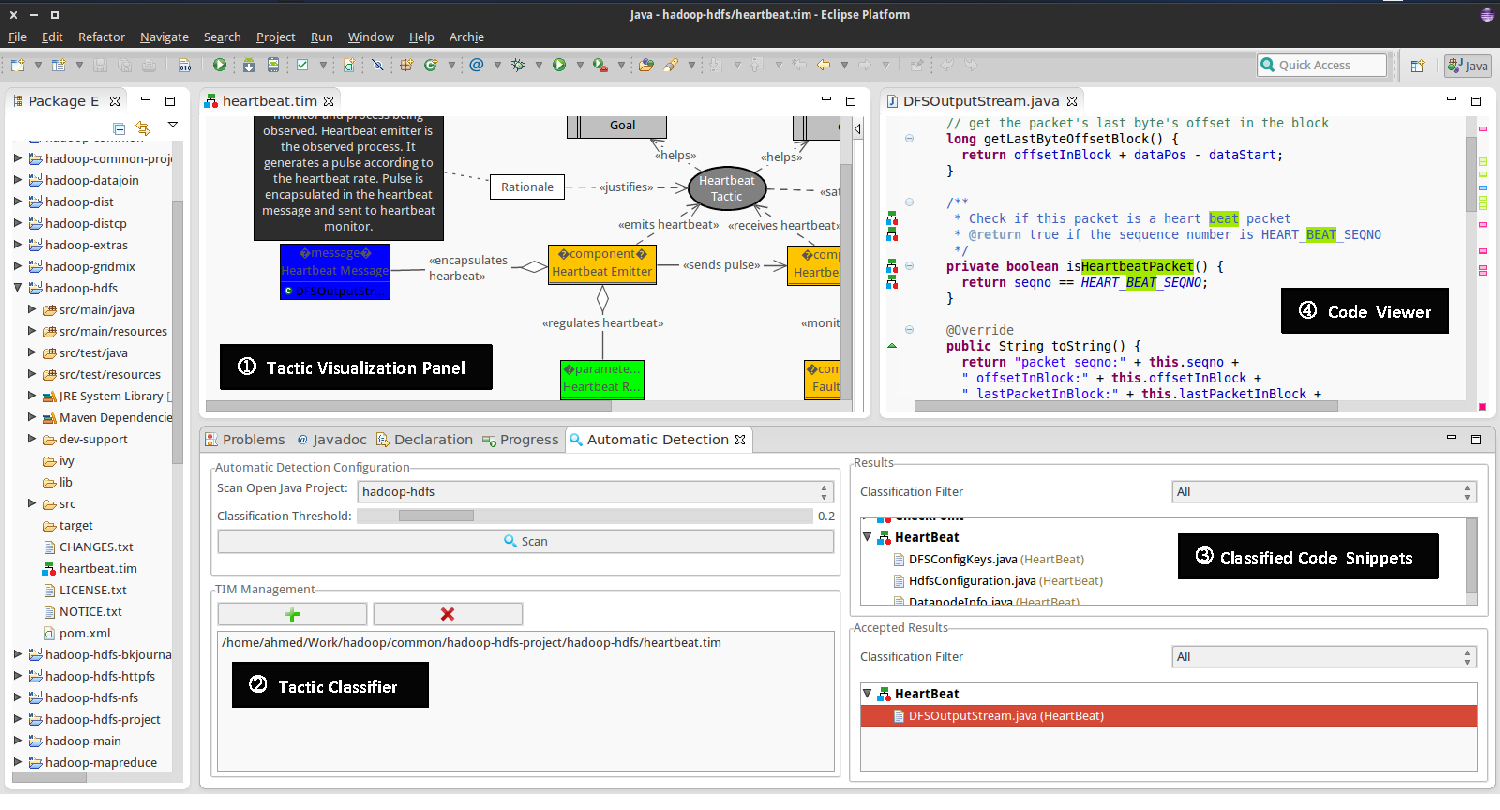
\includegraphics[width=0.9\linewidth]{./EclipseView}
\caption{A screen-shot of Archie, depicting different features and dashboards}
\label{fig:EclipseView}
\end{figure}





%\section{Quality Driven Design Assistant}
\section{Quality Driven Design: Tactical Spikes}
Customer satisfaction in any software product is highly dependent on the extent to which quality concerns such as performance, security, reliability, and availability~\cite{kruchten2004} are addressed. In practice, a rich set of proven and re-usable architectural solutions in terms of tactics can be used to satisfy each specific quality attribute~\cite{bass:arch12}. Architectural tactics, come in many different shapes and sizes and describe solutions for a wide range of quality concerns~\cite{Hanmer}. For instance, reliability tactics provide solutions for fault mitigation, detection, and recovery. Performance tactics grant solutions for resource contention to optimize response time and throughput. Security tactics provide solutions for authorization, authentication, non-repudiation and other similar factors~\cite{Hanmer}. Such tactics are found prevalently across many software systems~\cite{ICSE2012}.

\subsection{Tactical Spikes}
Archie is built around the fundamental concept of~\emph{Tactical Spikes} which advocates iterative incremental implementation of quality concerns through adoption of individual tactics. For each development cycle, developers focus on a limited number of quality attributes. Tactical Spikes break the development of architecture and satisfaction of quality concerns into small sprints with each focusing on a specific quality attribute and a fine grained design decision which can be implemented independently from other choices. Satisfying quality concerns through Tactical Spikes is not a new idea and has been widely used in incremental design where the architecture emerges through several development cycles.

Although experienced developers are often fully aware of tactics that can be used to implement quality concerns, inexperienced developers tend to ignore the importance of quality attributes or adopt solutions that do not match the context of a problem~\cite{FSE2012}. To integrate agile design thinking into a developer's daily activities, Archie utilizes a knowledge base of architectural tactics and uses this resource to provide suggestions about architectural tactics which can be implemented to address each quality concern. Developers can search the catalogue of quality attributes in Archie and find associated architectural tactics which can be used to implement them. This provides an embedded design resource in the programmer's IDE. 

\subsection{Tool Support}
To implement the idea of Tactical Spikes, we first introduce the fundamental concept of a Tactic Traceability Pattern (TTP)~\cite{Mirakhorli:2011:TAS:1985793.1986014, ICSM11} and then discuss the related functionality. TTP was previously used in maintaining the architecture of safety critical systems. It captures the context that a tactic can be used in, the design knowledge about the tactic, and primary conceptual roles to implement an architectural tactic. For the ~\emph{heartbeat} tactic (Figure~\ref{fig:HB}), the TTP indicates that this tactic can be used to address reliability and availability goals. The primary roles of this tactic include~\emph{emitter},~\emph{receiver}, and~\emph{health monitor}. 

\begin{figure}[tbph]
\centering
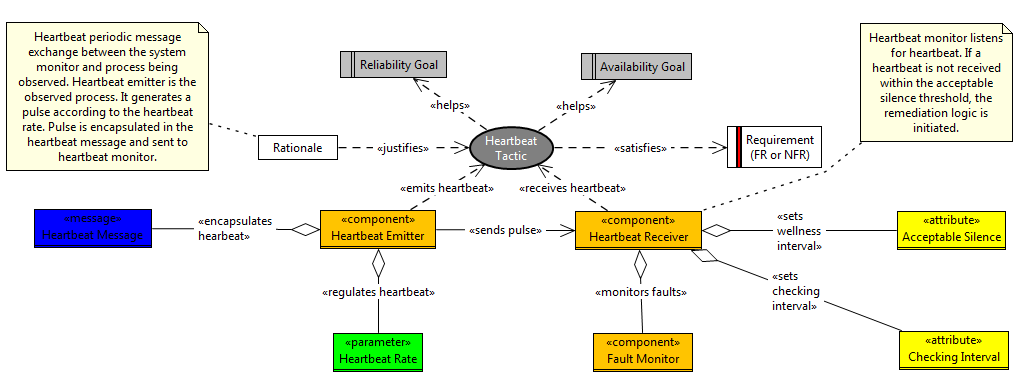
\includegraphics[width=0.9\linewidth]{./HB}
\caption{HeartBeat Traceability Pattern: Helping Developer to Better Adopt and Implement a Tactic}
\label{fig:HB}
\end{figure}


Furthermore, a TTP captures the relationships between these roles i.e. an emitter component sends messages to a receiver, while a health monitor takes actions if the monitored component fails. Lastly, a TTP also captures the underlying rationales for using the tactic which typically come in the form of a description that explains the quality concern being addressed. Each of the provided TTPs are initially populated with a set of default rationales. For example, in the case of heartbeat, these are related to reliability of a critical component. A user can modify rationales and also add references to relevant requirements. Archie ships with a basic set of TTPs including heartbeat, audit, authorization, resource pooling, and scheduler; however a user can utilize Archie's drag-and-drop modeling features to create customized TTPs.


The idea of Tactical Spikes are supported by TTP artifacts. Whenever developers want to implement a quality concern, they can look at the catalogue of TTPs in Archie and find the appropriate tactics which can be used to address their interested quality requirements. Furthermore, they would get an initial idea about which conceptual roles are involved when implementing the tactic. TTPs are modifiable artifacts (models), the developers can revise a TTP and document their micro design using basic UML modeling notations, they can also connect the tactical roles in the TTP to the source code. This can be done simply by selecting a segment of code and using mouse clicks to map it to either the entire TTP or to a specific role. Once the TTP is connected to the source code, it can provide a visual framework for communicating underlying architectural knowledge with other developers.







\section{On Demand Detection of Tactical Spikes}
Archie utilizes information retrieval and machine learning techniques to automatically detect architectural decisions from source code. The detection engine implements a set of classification techniques and each classifier is trained using code snippets representing different architectural tactics collected from hundreds of high-performance, open-source projects~\cite{FSE2012,ICSE2012,Dissertation}. In the training phase the classifiers learn the terms, method and variable names, and development APIs that developers typically use to implement each tactic. These terms are used during the classification phase to calculate the likelihood that any given source file implements a tactic. The accuracy of the tactical spike detection technique is evaluated through several experiments which indicate our technique is capable of returning reliable results. The details of our detection engine, the classification formula and accuracy metrics are described in several previous works~\cite{Dissertation,ICSE2012}. 

\begin{figure}[tbph]
\centering
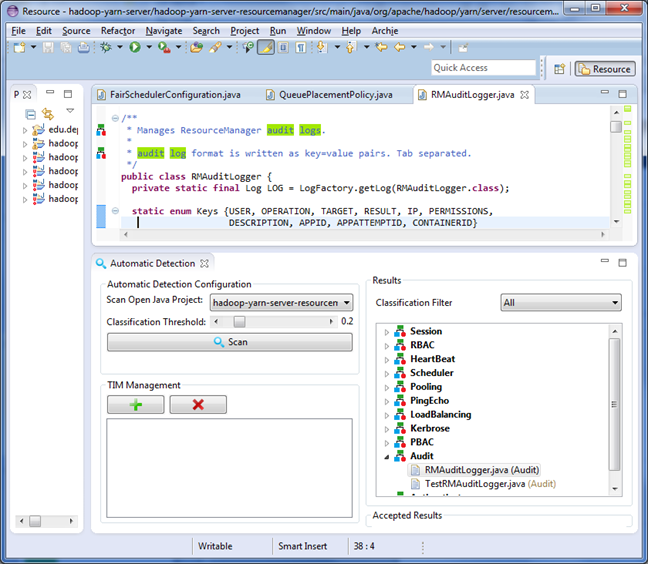
\includegraphics[width=0.9\linewidth]{./Detect}
\caption{Detected Tactical Spikes in Apache Hadoop Yarn Project}
\label{fig:Detect}
\end{figure}

Figure~\ref{fig:Detect} shows a screenshot of Archie where the classifiers are launched against the code in an Eclipse project. Several different architectural tactics are discovered in the source code of the Apache Hadoop Yarn project and categorized based on tactic type. Each category includes all the source files contributing to the implementation of each tactic. Furthermore, Archie highlights the method names, APIs and comments related to the tactic. For example, in Figure~\ref{fig:Detect} comments about audit trails are highlighted which helps developers understand why this file is considered tactical.

This feature will help developers to better understand the current state of implemented tactical spikes. This is especially useful when a new developer joins the team and they need to quickly comprehend the architectural choices behind the source code or when developers alter a new module of software which they have not worked on previously. Furthermore, this auto-detection engine can assist developers in more easily documenting their previous tactical spikes. Initially they can detect and recover architectural tactics in the source code, and then use the previously described feature of TTPs and connect these source files into a visual and informative representation of tactics. The visualization and documentation of tactical spikes as TTPs increases program comprehension and design communication which significantly reduces the effort to maintain such models compared to traditional approaches.

\section{Visualize Architecturally Significant Code}
Architectural decisions often exhibit complex and cross-cutting 
impacts upon the design, therefore communicating this information textually or socially can be quite challenging. Archie's visualization feature helps developers understand underlying design decisions within the context of the design and/or code. This can be especially helpful in agile projects where~\emph{no time for training} is a common occurrence~\cite{SEI_MaximumAwesome_url}  and design knowledge is primarily shared through social mechanisms such as pair-programming and regular meetings. When using Archie, a developer can automatically generate a view of the system illustrating tactics implemented in the source code and the files involved in the implementation.

\begin{figure}[tbph]
\centering
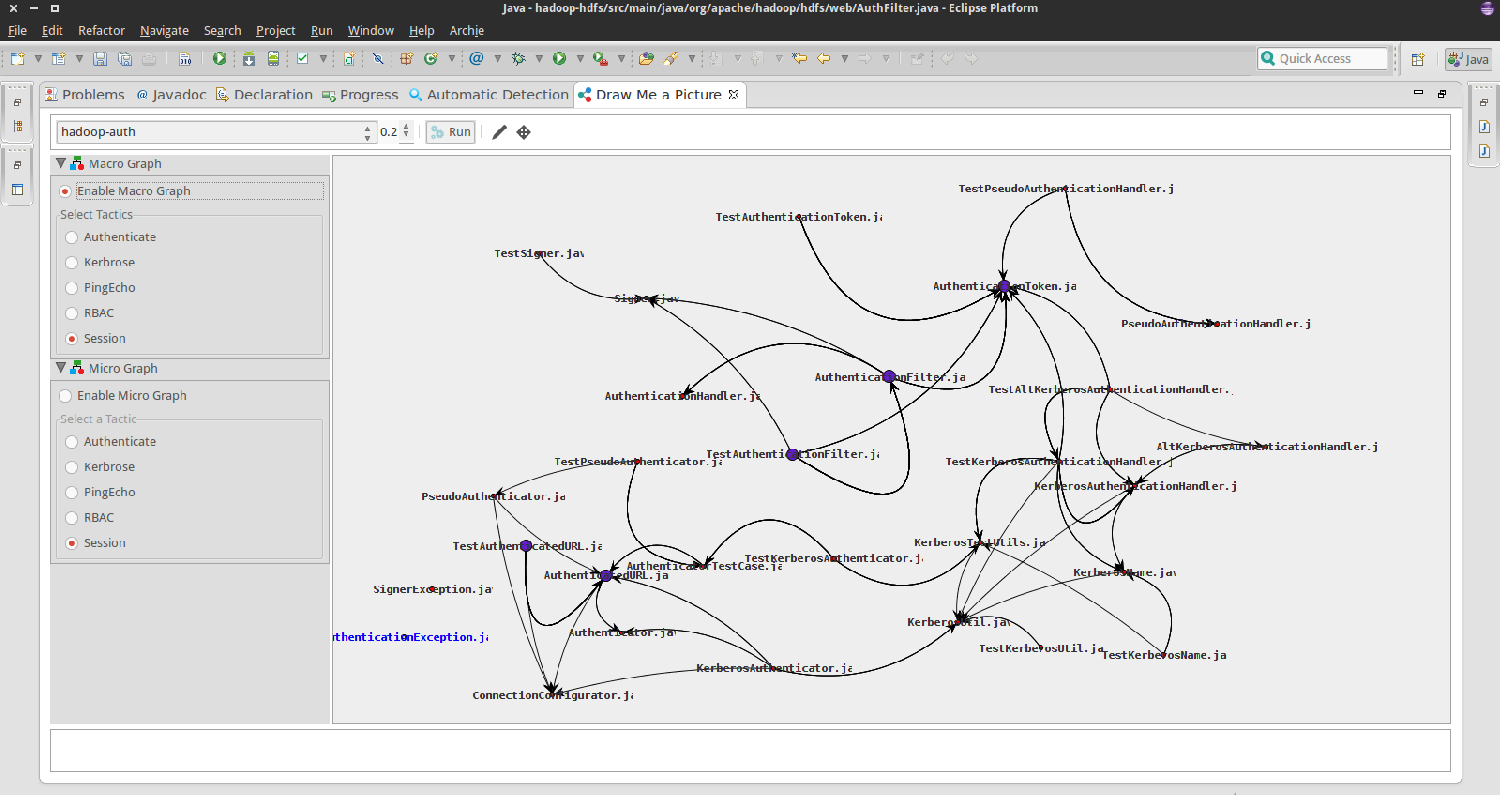
\includegraphics[width=0.9\linewidth]{./Visual1}
\caption{Visualization of Secure Session Management tactic Hadoop HDFS }
\label{fig:Visual1}
\end{figure}

Figure~\ref{fig:Visual1} depicts an automated visualization of secure session tactic in Hadoop HDFS subsystem. This view shows the source files involved in the implementation of tactic. In another example (Figure~\ref{fig:Audit}), we illustrate how Audit Trail tactic is implemented in Hadoop HDFS project, as well as the test files implemented to test this tactic. 

\begin{figure}[tbph]
\centering
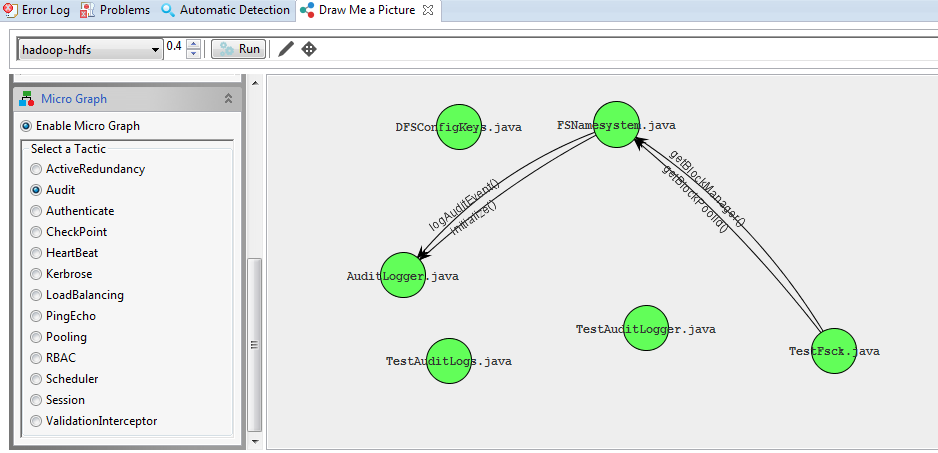
\includegraphics[width=0.9\linewidth]{./Audit}
\caption{Visualization of Audit Trail tactic and related test cases in Hadoop HDFS}
\label{fig:Audit}
\end{figure}
 

Archie provides features to help developers quickly create actionable models of tactical spikes. In this scenario, a developer may use Archie's automatic detection engine to locate implemented tactical spikes, and then connect these code snippets into TTPs. Establishing connections between source files and elements of TTPs requires only a single click. These features provide an easy and fast approach for creating rich architectural models during development. Furthermore, since these models are integrated with source code, any new programmer can open them in the programming IDE and understand the design decisions behind the code, the driving requirements, and the rationales behind design choices. Since TTPs can be customized, developers can add their own notes and elements into the model and communicate it with other developers on the team.



\begin{figure}[!t]
\centering
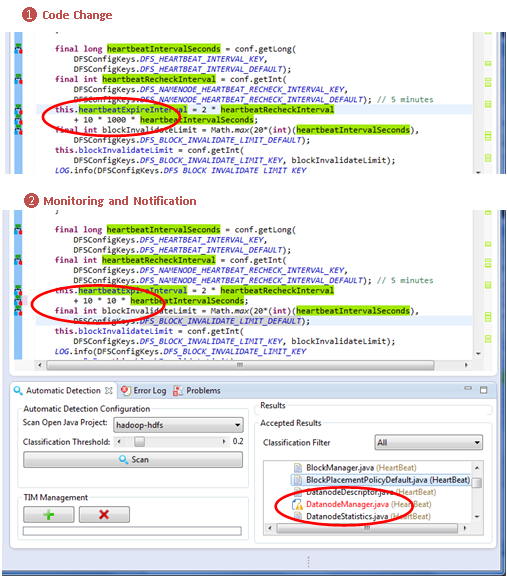
\includegraphics[width=0.99\linewidth]{./Monitoring}
\caption{An architecture protection scenario}
\label{fig:Monitoring}
\vspace{-16pt}
\end{figure}

\section{Decision Ownership and Accountability}
Large software systems are typically created by numerous developers. Files may be created and maintained by a single developer, or through a collaborative effort by many. Code ownership may be defined as the individual(s) who are primarily responsible for the creation of an application component~\cite{Rahman:2011:OED:1985793.1985860}.

A single developer acting as the primary owner of a component has several potential benefits. The first is that code ownership leads to high quality results through pride of workmanship and is easier to hold individuals accountable for the creation and maintenance of the component. Research has also shown that more developers working on a single component typically leads to more defects~\cite{Raymond:2001:CBM:560911}. However, owned code may suffer due to lack of external review since there may be less people examining it and may therefore hinder the discovery of problems~\cite{Rahman:2011:OED:1985793.1985860}. 

In practice there are several different models of code ownership. As defined by fowler~\cite{fowler_codeownership} the three levels of code ownership range from strong include, strong weak, and collective. Archie extends this notion to Design Ownership and provides an infrastructure for the developers to sign a tactical spike and be accountable for developing, testing, extending and maintaining related code snippets.

All architecturally significant code which has been mapped to TTPs or automatically detected by Archie are monitored for change activity. \emph{Archie} integrates an event-based traceability engine where all the tactical classes are registered with the event server, and the owner of tactical spikes is registered as a subscriber. Whenever a user modifies architecturally significant code, a notification event is triggered and the owner is notified. The developer making changes is also sent a message in the warning list depicting a visual representation of the underlying architectural. Figure~\ref{fig:Monitoring} depicts what the developer sees on a class that implements heartbeat emitter functionality in Hadoop~\emph{dataNode}. 

 The monitoring system highlights all tactic-related code, using a different color for each tactic. In this example, the~\emph{heartbeat}-related code is highlighted. The heartbeat TTP is concurrently shown to the developer that code in~\emph{datanode.java} serves as the heartbeat emitter, and that it sends heartbeats to~\emph{HeartBeatManager}. Along with this refactoring a message is sent to the owner of Heartbeat tactic in the system. The owner is the developer who first implemented the tactic or identified themselves as the owner.



\section{Related Work}

Several other works have discussed the importance of design in agile software development. Wirfs-Brock~\cite{Wirfs-Brock:2010:SAD:1869542.1869630} spoke about the significance of agile developers having the ability to quickly understand design problems and make timely decisions about how to address the issue. 

While our work is innovative, there are a wide range of existing techniques that support agile software development. Spoelstra et al.\cite{Spoelstra:2011:SRA:1982185.1982255} proposed a conceptual management tool for supporting software reuse in agile software development using a components derived from the Software Process Improvement (SPI) framework by Niazi et al.\cite{Niazi:2005:MMI:1045926.1045932}. Their tool utilizes maturity levels and reuse practices in order to create a reuse maturity model. However, none were specifically focused on agile architecture development. There is a wide range of other tools supporting agile software development including tools for software project management and planning~\cite{Petersen:2008:APT:1379092.1379101, Dhlamini:2009:IRM:1562741.1562745}, and modeling~\cite{Buchmann:2012:TTS:2467307.2467310}. 

Several researchers have attempted to address architectural challenges through developing techniques for organizing, documenting or modeling architectural decisions. The Architecture Design Decision Support System (ADDSS)\cite{ADDSS}, Process based Architecture Knowledge Management Environment (PAKME)\cite{PAKME}, and Architecture Rationale and Element Linkage (AREL)\cite{AREL} are examples of these. However, these approaches are not adopted to the agile development mindset, and fail to address the scalability issues of managing potentially large numbers of architectural decisions.  They also fail to connect design decisions to code, and/or provide little support for actually utilizing this knowledge during software maintenance. 





\section{Conclusion}
While Archie's primary goal was to support secure software development, the automated features of Archie make it a unique tool for agile teams as well. The primary contribution of Archie is in the area of architectural centric support and preservation of architecture through detecting and tracing architectural concerns, and then using these trace links to keep developers fully informed of underlying architectural knowledge.

\section{Acknowledgments}
Archie was partially funded by the U.S. Department of Homeland Security.

\bibliographystyle{spmpsci}
\bibliography{XP2015}



\end{document}
